
\documentclass[a4paper]{article}
\usepackage[english]{babel}
\usepackage{enumitem}
\usepackage{mathrsfs}
\usepackage{amsmath}
\newcommand\norm[1]{\left\lVert#1\right\rVert}
\usepackage{graphicx}
\graphicspath{ {images/} }
\usepackage[makeroom]{cancel}
\usepackage{amssymb}

\begin{document}
\title{SSD Questionary}
\author{Enrique C. Toomey}
\date{\today}
\maketitle


\section{Questions 1.1}
\begin{enumerate}[label=\emph{\alph*)},series=preguntas1_1]
  \item % a) What are the three main application areas of distributed space systems? Name some key specific applications where breakthroughs are expected in the near future
    The main three application areas of distributed space system are:
  \begin{itemize}
    \item Space Science (Solar system exploration, Astronomical search of origins)
    \item Planetary science (synthetic aperture radar interferometru, gravity mapping, etc.)
    \item Technology (On orbit servicing and assembly, Humman exploration technology)
  \end{itemize}
  One key specific aplication where breakthroughts are expected in the near future is space debris elimination.

  \item % b)What are the main mission architectures of distributed space systems according to inter-satellite distance and requiredcontrol accuracy?
    We can distinguish four different distributed space system's  mission architectures according to the inter-satellite distance adn required control accuracy:
  \begin{itemize}
    \item In the lowest inter-satellite distance and highest accuracy required, we have Rendezvous and docking.
    \item In the largest inter-satellite distance and least accuracy required we have constellations, such as GNPS.
    \item In between Rendevous adn Constellations, we have a broad band of mission architectures grouped under the Formation flying mission architecture.
    \item Least of all, we have swarm and fractionated spacecraft mission architecture, requiring low control accuracy for a wide band of inter-satellite dintances.
  \end{itemize}

  \item % c) What are the main mission architectures of distributed space systems according to inter-satellite distance and required control accuracy?
    The key differences between historic, contemporary, and future distributed space systems are that historically, misions where generously founded, ment for short duration, and control was always made from gound (no autonomous navigation). Nowadays missions are ment to be long-duration, cost-efficient and autonomous. Future distributed space system will tend towards miniaturization and standarizartion, using off the shell hardware and easily replacesable technology in order to keep on track with a fast technological development. So we can say that we are going from big and expensive to small and cost-effective, from ground-control to autonomous, and from a single standalone satellite conception to a distributed system paradigm.

  \item %d) Name at least 2 past and 2 upcoming missions based on distributed space systems and identify their main objectives 
    Past distributed space system missions:
    \begin{enumerate}[label=\arabic*., series=pregunta4]
      \setlist[enumerate]{resume}
      \item Apollo mission with its lunar module docking manouver.
      \item (More recently) Tamdem-X mission using two SAR satellites in order to build a 3D model of earth.
    \end{enumerate}

    Upcomming missions:
    \begin{enumerate}[resume*=pregunta4]
      \item New world observatory: use un combination a telescope satellite and a shield satellite which will cast the shadow of a star to the telescope, making the second one able to watch planets around the star, that they would be otherwise obscured by the star ligth.
      \item Earth observations constellations using low-earth orbit satellite which would communicate between themselves in order to achive earth observations objective, solve communications downlink bottle-necks, distributed fuel consumption to maintain optimar constellation shape.
    \end{enumerate}

  \item % e)What are the typical fuel-use drivers in distributed space systems?
    Tipical fuel-use drivers are:
  \begin{itemize}
    \item Mission requirements.
    \item Initial conditions
    \item Navigation uncertainty
    \item Actual errors
    \item Dynamical process noise
  \end{itemize}

  \item % f) What are the typical fuel-use drivers in distributed space systems?
    Formation control strategies:
  \begin{itemize}
    \item Proportional-derivative
    \item Linear quadratic regulation
    \item Linear matrix inequalities
    \item Lyapunov
  \end{itemize}

  \item % g) What is the most common formation control strategy used in practice? Why?
    The most common formation control strategy used in practice is using thrusting schemes because they are reliable and can be accurately calculated on ground. 

  \item % h) What are the relative navigation approaches adopted in the PRISMA technology demonstration mission?
    The negative navigation approaches adopted in the PRISMA mission are:
    \begin{itemize}
      \item Vision Based navigation.
      \item Autonomous formation flying. 
   \end{itemize}

\end{enumerate}

\section{Quations 1.2}
\begin{enumerate}[label=\emph{\alph*)}]
  \item % a) Name the fundamental plane, origin, and axes pointing for ECI, Perifocal, ECEF, RTN, and Polar rotating coordinate systems
    \begin{itemize}[label=\textbullet]
      \item ECI:
	\begin{itemize}
	  \item Plane: Equatorial plane.
	  \item Origin: earth center of mass.
	  \item Axes pointing: x vernal equinox, z earth rotation axes.
	\end{itemize}
      \item Perifocal:
	\begin{itemize}
	  \item Plane: orbit plane
	  \item Origin: orbit focal point
	  \item Axes pointing: x focal to periasis, z normal to orbit.
	\end{itemize}
      \item ECEF:
	\begin{itemize}
	  \item plane: ecliptic plane 
	  \item origin: earth center of mass.
	  \item axes pointing: x intersection between greenwitch latitud  and equator plane
	\end{itemize}
      \item RTN:
	\begin{itemize}
	  \item plane: orbit plane
	  \item origin: satellite
	  \item axes pointing: x = r(position), y = v(velocity)
	\end{itemize}
      \item Polar rotation coordinates:
	\begin{itemize}
	  \item plane: ecliptic plane
	  \item origin:
	  \item axes pointing:
	\end{itemize}
    \end{itemize}

  \item % b) What are the assumptions behind the restricted two-body problem?
    The assumptions behind the restricted earth two body problem are that the secondary mass is negligible compared to m1, and that m1 has a perctly spherical gravitational field. There's no external forces.

  \item % c) What is the fundamental orbital differential equations? What is its solution in polar coordinates?
    Fundamental orbital differential equations:
    \[\ddot{\vec{r}}+\mu\frac{\vec{r}}{r^3}=0\]
    Polar coordinate solution:
    \[r = \frac{p}{1+e\cdot\cos{f}} \qquad \textrm{with:}\]
    \[p = \frac{h^2}{\mu},~~ e=\sqrt{1+\frac{2e h^2}{\mu^2}} ~~ \textrm{and} ~~ f=\theta-\omega\]
    
  \item % d) What are the steps necessary to derive the solution of the orbital differential equations in inertial coordinates?
    To derive the solution in inertial coordinates first we construct the position vector in the perifocal axis:
    \[[r]_{\mathscr{P}}=[r\cos{f};r\sin{f};0] = \]
    Then, we use the three orbit parameters that define the orbit in the inertial frame to rotate the position vector define in the pericoal axis to the inertial axis:
    \[ [r]_{\mathscr{I}} =T_{\mathscr{P}}^{\mathscr{I}}~(\omega,i,\Omega) ~[r]_{\mathscr{P}}\] 
  
  \item % e) What are the steps necessary to derive the solution of the orbital differential equations with time as independent variable?

    
  \item % f) Which orbit elements are not conserved in the restricted two-body problem?
    The true anomaly $f$  or the mean anomaly $M$
    
  \item % g) Besides the orbit elements, what key quantities are conserved in the restricted two-body problem?
    Angular momentum and energy.
    
  \item % h) Can the Keplerian orbit elements become degenerate? Show some representative cases. What can be done to circumvent this problem?
    Yes, for certain orbits the solutions becomes singular (for example, ciruclar orbits -$e=0$-, or equatorial orbits)
   
  \item % i) Problem
    \[\vec{r} = 2 \hat{i}\]
    \[\vec{v} = \frac{-1}{\sqrt{2}}+\frac{1}{\sqrt{2}}\hat{j}\]
    \[\vec{h} = \vec{r} \times \vec{v}= \frac{2}{\sqrt{2}}\hat{k} \rightarrow ~ h ~ \textrm{is aligned with Earth's rotating axis, so the orbit is equatorial.}\]
    To evaluate if the orbit is circular, elliptical, parabolic or hyperbolic we check the value of $E$:
    \[E = -\frac{\mu}{2a} = \frac{v^2}{2}-\frac{\mu}{r} = \frac{1}{2} - \frac{1}{2} = 0 \quad \rightarrow \quad \textrm{The orbit is parabolic.}\]

\end{enumerate}


\section{Questions 2.1}
\begin{enumerate}[label=\emph{\alph*)}]
  \item %a) How do we solve the fundamental differential equations in the presence of perturbations?
    There are two aproaches: asuming an harmonical potential perturbation force (Lagrange Planetary Equations), or directly integrating the orbit parameters variations due to arbitrary perturbations forces expressed in the RTN frame (Gauss variational equations).
  \item %b)  we expect to only spend a tiny fraction of this in the next few years.
    The method of variation of parameters cosist on the following steps:
    \begin{itemize}
      \item Take the homogeneous solution of the differential equation.
      \item Take the integration constants of the 'unperturbed' motion.
      \item Express these constans as a function of time.
      \item Introduce ad-hoc constrains to simplify equations.
      \item Solve for new, now time-dependent parametes.
    \end{itemize}
  \item % c) What are the Lagrange’s and Gauss variational equations? Under which assumptions are they derived? What are the main differences?
    Both sets of equation uses the oculating constrains in order to obstain the three extra degrees to solve the VOP problem:
    \[\frac{\partial f}{\partial oe} \dot{oe} = 0\]
    This means that the trajectory in the inertial configuration space is always tangential to an 'instantaneous' elipse (or hyperbola) defined by the instantaneous values of the time-varying orbital elements.
    \begin{itemize}
      \item Lagrange variational equations: In presence of a conservative, position-only dependent perturbing potential, VOP (variation-of-parameters) leads to the LPE. LPE uses geo-potential expansion in spherical harmonics to model earth gravitational field.
	\[\frac{d\vec{oe}}{dt} = \mathscr{L}^{-1}\frac{\delta R}{\delta \vec{oe}} \]
      \item Gauss variational equations: does no assumption on $\vec{d}$
	\[\dot{oe}=\frac{\partial oe}{partial v} d\]
    \end{itemize}
  
  \item % d) How can we incorporate higher order geopotential coefficients in our solution? How can we incorporate atmospheric drag in our solution? How can we incorporate impulsive maneuvers in our solution?
    Perturbation forces $d$ due to the geopotential $R$ are computed through:
    \[ d = \frac{\partial R}{\partial r}\]
    where $R$ can be modeled as a series of Legendre polynomials $P_k$:
    \[ R = -\frac{\mu}{r} \sum_{k=2}^{n}{J_k \left( \frac{Re}{r} \right)^k P_k(\cos{\phi})}\]
    where $\cos{phi}=\sin{i}\cdot\sin{f+w}$ and $P_k(x) = \frac{1}{2^k !k}\frac{d^k}{dx^k}\left[(x^2-1)^k\right]$. The larger $n$ is (number of terms in the series), the higher the order of the potential model used is, leading to more realistic earth modelling.\\
    Atmospheric drag can be incorporated using gauss variational equations, with osculating constrains. Acceleration $d$ due to drag is calculated through:
    \[ a_D = -\left(\frac{A}{m} \right) C_D \rho \frac{v^2}{2}~\hat{i}_v \]
    As th versor $\hat{i}_v$ is not aligned with the RTN frame, the following rotation matrices may be use:
    \[ \left( \begin{array}{c} a_r \\ a_t \end{array} \right) = \frac{1}{\sqrt{1+e^2+2e\cos{f}}} \left[ \begin{array}{c c} 1+e\cos{f} & e\sin{f} \\ -e\sin{f}  & 1+e\cos{f} \end{array} \right]  \left( \begin{array}{c} a_{D\perp} \\  a_D \end{array} \right) \]
    Maneuver can be modeled as instantaneous variations of velocity, which cause instantaneous variations in the relative orbit elements.
  \item % e) Describe the key effects of J2, drag, and impulsive maneuvers on the orbit solution
    J2 effects can be decompose in short term and long term oscilations, and secular effects. Secular effects affects $\Omega$, $\omega$ and $M_0$ in the following way:
    \begin{minipage}{\textwidth}
      \begin{flushleft}
	\[ \frac{d\bar{\Omega}}{dt} = -\frac{3}{2} J_2 \left( \frac{Re}{\bar{p}} \right)^2 \bar{n} \cos{\bar{i}} \]
	\[ \frac{d\bar{\omega}}{dt} = \frac{3}{4} J_2 \left( \frac{Re}{\bar{p}}\right)^2  \bar{n} (5\cos{\bar{i}}^2 -1) \]
	\[ \frac{d\bar{M_0}}{dt} = \frac{3}{4} J_2 \left( \frac{Re}{\bar{p}}\right)^2  \bar{n} \sqrt{1-\bar{e}^2} (3\cos{\bar{i}}^2 -1) \]
      \end{flushleft}
    \end{minipage}

    Atmospheric drag's main effect is the semi-mayor axis $\bar{a}$  and excentricity $\bar{e}$ reduction (orbits tend to be circular). It also introduce periodic effects on $\omega$, $M$ and $e$.\\
    Maneuvers can affect any of the six orbital elements:
    \begin{itemize}
      \item Cross-track maneuvers affects $(\bar{i},\bar{\Omega},\bar{\omega})$.
      \item Along-track maneuvers affects $(\bar{a},\bar{e},\bar{\omega},\bar{M_0})$.
      \item Radial maneuvers affects $(\bar{a},\bar{e},\bar{\omega},\bar{M_0})$, though less strongly than along-track maneuvers.
    \end{itemize}

  \item % f) What are the inclinations which remove secular effects of J2 on the orbit elements?
    For polar orbits $(i=90^o)$, $d\bar{\Omega} / dt$ effects disapear. To remove $\bar{\omega}$ and $\bar{M_0}$ effects, $i$ must be equal to $\cos^{-1}{\sqrt{1/5}}$ and $\cos^{-1}{\sqrt{1/3}}$ respectively.
 
  \item % g) What are the secular effects of atmospheric drag on the orbit elements?
    Secular effects of atmospheric drag are:
    \[ \frac{d\bar{e}}{dt} = -\left(\frac{A}{m} \right) C_D \rho \bar{e}; \qquad  \frac{d\bar{a}}{dt} = -\left(\frac{A}{m} \right) C_D \rho \frac{v^3}{\bar{a}\bar{n}^2} \]

  \item % h) Do out-of-plane impulsive maneuvers affect the in-plane orbit motion? If yes, is this conclusion still valid if we use the so-called longitude λ = ω + M0 + Ωcos(i) to describe the phasing of the spacecraft along its orbit?
    Yes, out-of-plane impulse maneuvers affect $\omega$ in the following way:
    \[\Delta\omega = -\frac{\Delta V_h r \sin{f+\omega}\cos{i}}{h\sin{i}} \]
    In the case we use $\lambda = \omega+M+\Omega\cos{i}$:
    \[\arraycolsep=1.4pt\def\arraystretch{2.2}
    \begin{array}{c c l} \Delta\lambda|_{\Delta v_h} &=& \Delta \omega|_{\Delta v_h} + \cancelto{0}{\Delta M|_{\Delta v_h}} + \Delta \Omega|_{\Delta v_h} \cos{i} - \Omega \sin{i} \Delta i|_{\Delta v_h} \\
	&=& \cancel{-\frac{\Delta V_h r \sin{f+\omega}\cos{i}}{h\sin{i}}}+ \cancel{\frac{\Delta V_h r \sin{f+\omega}\cos{i}}{h\sin{i}} } - \frac{\Omega \sin{i}\cos{f+\omega}r\Delta v_h}{h}  \\
    \Delta\lambda|_{\Delta v_h} &=& - \frac{\Omega \sin{i}\cos{f+\omega}r\Delta v_h}{h} \end{array}\] 

  \item % i) Where would you place a maneuver to change inclination only, how oriented in RTN? Where would you place a maneuver to change right ascension of ascending node only, how oriented in RTN? Where would you place a maneuver to change the semi-major axis, how oriented in RTN and w.r.t velocity?
    To change $i$ a cross-track maneuver in needed in the line of node $\theta = f + \omega = 0$. To change $\Omega$, the cross-track maneuver must be made $90^o$ from the line of nodes $(\omega+f=90^o$, not valid for polar orbits). To change the semi-mayor acis the maneuver must be made in the direction of the velocity vector (this may affect $e$, $\omega$ and $M_0$ also, but would not alter $i$ and $\omega$). In the RTN frame the maneuver is:
    \[a_R = \frac{e\sin{f}}{\sqrt{1+e^2+2e\cos{f}}} a_v \]
    \[a_N = \frac{1+ e\cos{f}}{\sqrt{1+e^2+2e\cos{f}}} a_v \]

\end{enumerate}

\section{Questions 2.2}
\begin{enumerate}[label=\emph{\alph*)}]
  \item %a) Describe two possible ways to simulate numerically the relative motion between formation-flying spacecraft including perturbations
    One way is to numerically integrate the dynamics of each spacecraft and then compute the difference. Another way is to write de dynamic equation in terms of diferential position or diferential orbital elements, and numerically integrate those variables. This second aproach require knowing the solution to the equation of motion for one of the spacecraft, called the chief spacecraft.

  \item %b) Describe two possible ways to compute the relative position and velocity of formation-flying spacecraft in the RTN frame
    Relative position and velocity can be compute directy by diferenciating the position and velocity of each spacecraft, both expressed in the same frame. Another way is by direcly solving the relative equation of motion, generally expressed in the chief's centered RTN fram.
  \item %c) What are mean and osculating orbit elements? Why are mean orbit elements useful? How can we convert from osculating to mean orbit elements? And from mean to osculating orbit elements?
    Osculation orbital elements are the orbital elements corresponding to the instantaneus position and velocity, slution of the non-homogenious kepler equations. Mean orbital elements are obtain from osculating elements using the averaging theory (averaging through a whole orbit). It is often convenient to specify the initial conditions of the satellite orbit though the mean orbital elements, since the formation design/control is tipically done using this parameters. Mean orbital elements canbe transform to osculating orbital elements (and then to position and velocity) via the Brower Theory.

  \item %d) What are the assumptions behind the nonlinear equations of relative motion? Describe the meaning of the left and right hand side of the equations.
    No assumptions are made when developing the non-linear equations of relative motion. The left hand terms represent the inertial acceleration of the relative position vector. The right hand side stands for the diference gravitational force between both spacecrafts.

  \item %e) Do they admit a closed-form solution, in what state representation? Do they admit equilibria, which ones?
    For non-constant angular velocity $\ddot{\theta_0} \neq 0$, non-linear equations of relative motion admit a single relative equilibrium at $x=y=z=0$ (chief and deputy are in the same position).They do no admit a close a closed-form solution in any state representation.
  \item %f) What is commensurability and why is it important for formation-flying? How do we derive the energy matching condition and what can be used for?
    Two elliptic orbits are commensurable if their periods $T_1$ and $T_2$ follow the relation:
    \[ \frac{T_1}{T_2}=\frac{m}{n} \qquad \mathrm{with}~m,n~\epsilon~\mathbb{E}\]
    this is related with the orbit energy through the follow equation:
    \[ T = \frac{\pi\mu}{\sqrt{2(-\mathcal{E})^{3}}}\qquad \rightarrow \qquad \frac{\mathcal{E}_2}{\mathcal{E}_1}=\left( \frac{m}{n}\right)^{3/2} \]
    Orbit commnesurability can be use to obtain a simple algebraic constrain on initial conditions which guaranteed bounded relative orbits.
  \item %g) What are the key simplifications of the equations of relative motion when considering a circular reference orbit? What are the new equilibria? Show that they are consistent with the energy matching condition. What is libration?
    Considering a circular chief's orbit, the following simplifications can be done: $\dot{\theta_0}=n_0$, $\ddot{\theta_0}=0$ and $r_0=a_0=cte$. This leads two a new equilibrium condition given by:
    \[ z = 0,~(x+a_0)^2+y^2 = a_0^2\]
    This means that the deputy is in the exact same orbit that the chiefs, but with a different value of $f$. As the orbits have the same semi-mayor axis $a_0$, the energy mathching condition is satisfy. From a dynamical systems perspective, small perturbations near equilibria generate periodic orbits about the equilibria. This periodic motion is called ``libration''.

  \item %h) What are the key simplifications of the equations of relative motion when considering a circular orbit and small separations of the co-orbiting spacecraft as compared with the orbit radius? What are the assumptions behind the HCW equations? How are they derived? What characteristics make the HCW equations linear and decoupled? What are the new equilibria? Are the consistent with previous findings and the energy matching condition?
    When a small separation between spacecrafts is considered in addition to the circular orbit simplification, the equations of motion can be linearize about the origin of the chief-fixed frame, obtaining the HCW equations. This is done expanding the right-hand side of the equations into a Taylor series about the origin and retaining first terms only. The equations obtain have the out-of-plane$(z)$ motion decoupled from the in-plane motion $(x,y)$. The new equilibria condition is obtain by forcing $x=z=0$. This means that the deputy is located aligned with the along-track direction of the chief spacecraft. This conditions is due to the linearization, in which the circular orbit was aproximated by the tangent in the chiefs centered frame. This conditions does not satisfy the energy mathching condition, because $a$ is not the same for both spacecrafts.

\end{enumerate}
\section{Questions 3.1}

\begin{enumerate}[label=\emph{\alph*)}]
  
  \item % a) Describe the key characteristics of the solution of the HCW equations? Link eigenvalues to periodic and secular modes
    The solution of the HCW equations have the following characteristics:
    \begin{itemize}
      \item $x,y$ movement are decoupled of the $z$ movement.
      \item The $y$ component of the equation of motion has a linear drift depending on the term: $[6nx(0)+3\dot{y}(0)]t$
      \item We can relate the periodic oscilation in the three equations with complex eigenvalues of the 6x6 A matrix.
    \end{itemize}
  \item % b)What are the equilibria of the HCW equations? How do they compare to ones of the nonlinear equations? Are there possible contradictions? How do you explain those?
    The equilibria of the HCW equation are every solution with the $x=z=0$, that means, the deputy in the RTN $y$ axis. For the non-linear case, the equilibria is satisfy when the deputy is placed in the same orbit than the chief (same mayor axis). The difference between both solutions is due to the linearization of the orbit, which is aproximated by its tangent.
  
  \item % c) Describe the solution of the HCW equations in amplitude/phase form. Derive the eccentricity of the relative orbit projected in RT. When do we obtain an elliptical relative orbit when projected in RN?
    The magnitud-phase solution of the HWC equations have same phase $\alpha_x$  for x and y motion equation, having the same period. This is interpreted as a eliptic trayectory in the $x,y$ plane, with its center of motion shifted in the $y$ direction. We can obtain a 3D elipse if we force the z phase $\alpha_z$ to be equal to $\alpha_x$. The excentricity in the RT ($x,y$ plane) can be obtain from:
    \[ x(t)=\rho_x\sin{(nt+\alpha_x)}\]
    \[y(t)=\rho_y+2*\rho_x\cos{nt+\alpha_x)}\]
    \[x_2(t)+\frac{{(y-\rho_y)}_2}{2}=(\rho_x\sin{(nt+\alpha_x)})^2+(\rho_x\cos{nt+\alpha_x})^2=\rho_x^2\]
  The expresion obtained, as said before, corresponds to an elipse, whos mayor axis is $2\cdot \rho_x$ and minor axis $\rho_x$. Using this to calculate the excentricity:
    \[e=\sqrt{1-\frac{\rho_x^2}{4\rho_x^2}}=\frac{\sqrt{3}}{2}\]

  \item % d) Describe the solution of the HCW equations in amplitude/phase form. Derive the eccentricity of the relative orbit projected in RT. When do we obtain an elliptical relative orbit when projected in RN?
        The dificult in designing bounded (non drifting) relative orbits using HCW is that there is an inhereted drift caused by the linearization of the equation, cuadratically proportional to the distance between chief and deputy. Even with the non-drifting initial conditions of there is a drift from the ''real'' solution of the restricted two body porblem. This problem can be circumvent using the curvilinear coordinates $(\delta r,\theta_r,\phi_r)$. The HCW equations expresed in this coordinates have the exact same form than the ones obtained using cartesian coordinates.
  
  \item % e)How do we derive the linearized equations of relative motion for arbitrary eccentricity (Tschauner-Hempel, TH)? What are the similarities and differences between HCW and TH?
    The linearized equations of relative motion for arbitrary eccentricity are derived by first normalizing the RTN relative variables $x,y,z$, and incorpotaring a non-dimensial potential function $\mathscr{W}$ and $\mathscr{U}$ of the form:
   \[ \mathscr{W} = \frac{1}{1+e_0 \cos{f_0}} \left[ \frac{1}{2}(\bar{x}^2+\bar{y}^2+e_0 \bar{z}^2 \cos{f_0})-\mathscr{U} \right]  \]
   \[\mathscr{U} = -\frac{1}{\left[(1+\bar{x})^2+\bar{y}^2+\bar{z}^2 \right]^{\frac{1}{2}}}+1-\bar{x}\]
   Finally, instead of using the time as the independent variable, $f$ is used. The time derivative becomes:
   \[\frac{d(\cdot)}{dt}=(\cdot)'\dot{f}\]
   This enable us to write the general relative motion equation as:
   \[\bar{x}''-2\bar{y}''=\frac{\partial\mathscr{W}}{\partial\bar{x}}\]
   \[\bar{y}''+2\bar{x}''=\frac{\partial\mathscr{W}}{\partial\bar{y}}\]
   \[\bar{z}''=\frac{\partial\mathscr{W}}{\partial\bar{z}}\]

   Which can be linearized to:
   \[\bar{x}'' = \frac{3}{k} \bar{x}+2\bar{y}'\]
   \[\bar{y}''= -2\bar{x}' \]
   \[\bar{z}'' = -\bar{z}' \]
   where $k =  1+e\cos{f}$. The equations obtained have the same form than the HWC equations, except for term $1/k$ multiplying $\bar{x}$ in the first equation. 

  \item  % f) How do we derive the solution of TH (Yamanaka-Ankersen, YA)? What are the secular effects (unbounded relative orbit) and how can we remove them? Are there multiple combinations of initial relative position and velocity that provide bounded motion according to YA? What are the differences between no-drift conditions from TH and HCW?
      Yamanaka-Ankersen solution can be obtain by integrating the along-track motion to produce $\bar{y}'$, which is then substituted into the radial motion to obtain an uncoupled differential equation for $\bar{x}$. Solving for $\bar{x}$ enables to obtain  $\bar{y}$. The out-of-plane motion is already decoupled, and can be easily instegrated to obtain a simple harmonic oscilator.The solution is:
   \[\bar{x} = c_1 k \sin{f}+c_2 k \cos{f} + c_3 (2 - 3 e k I\sin{f})\]
   \[\bar{y} = c_4 + c_1 (1+1/k)\cos{f} - c_2 (1+1/k) \sin{f} - 3 c_3 k^2 I \]
   \[\bar{z} = c_5 \cos{f} + c_6 \sin{f}\]
   where $c_{1:6}$ are integration constants and $I = \int_{f(0)}^{f}{\frac{1}{(1+e\cos{f})^2}} = \frac{\mu^2}{h^3}(t-t_0)$. The terms constaining $I$ are the drifting terms, which can be remove by setting to 0 $c_3$. This leads to the following equation, which must be satisfy in order to guarantee no drift in the relative motion:
   \[k(f(t_0)) [\dot{y}(t_0)+\dot{f}(t_0)x(t_0)] + e \sin{f(t_0)}\cdot [\dot{x}(t_0) - \dot{f}(t_0)y(t_0)] + \dot{f}(t_0)x(t_0) = 0 \]
   \[ \qquad  \mathrm{with} \qquad \dot{f}(t_0) = \sqrt{\frac{\mu}{p^3}}k(f(t_0))^2  \]
   There are several combinations of initial position and velocity which satisfy this equations. In the case where $e=0$ and $f(t_0)=0$, the no drift conditions is equal to the no drift condition fot the HCW equations: $\dot{y}+nx=0$.
  
  \item % g) Describe the solution of the TH equations in amplitude/phase form. What are the differences with the solution of HCW? Can we obtain bounded and centered relative motion similar to the HCW’s solution? How?
   When expressed in amplitude/phase form, the non drifting solution has the following form:
   \[x = \rho_x \sin{f+\alpha_x} \]
   \[y = 2 \rho_x \cos{f+\alpha_x} \frac{1+\frac{e}{2}\cos{f}}{1+e\cos{f}} + \frac{\rho_y}{(1+e\cos{f})} \]
   \[z = \rho_z \frac{\sin{f+\alpha_z}}{1+e\cos{f}} \]
   The main difference with the solution of the HCW equations is the along-track bias term  $\frac{\rho_y}{(1+e\cos{f})}$, which can be remove imposing $\rho_y=e\rho_x\cos{\alpha_x}$,  and the $\frac{1+\frac{e}{2}\cos{f}}{1+e\cos{f}}$ term affecting the along-track motion, which leads to a non eliptic solution for the relative motion.
 
  \item % h) How would approximate the difference in semi-major axis between deputy and chief according to the HCW and YA?
  
\end{enumerate}

\section{Questions 3.2}

\begin{enumerate}[label=\emph{\alph*)}]
  \item % a) Why do we use orbit elements to describe relative motion? How do we derive a linear mapping between Hill coordinates
        %    and combinations of orbit elements? What are the specific assumptions adopted?
    Using orbit elements to describe relative motion is analog to using curvilinear variables: When linearizing, the equations of motion obtained are a better aproximation to the non-linear ones. Also, for the restricted two body problem, both deputy and chief orbit elements are constant (with exception of $M$ or $f$), so their difference will also be constant. In order to map the relative orbit elements to Hill coordinates, we use the linear mapping. The deputy position vector is expresed in the chief RTN set of coordinates using the rotation matrix from chief to inertial, and from inertial to deputy. Linearizing about the chief orbits, we can express the deputy to inertial rotation matrix as:\\
    \[[ND]=[NC]+[\delta NC]\]
    The variation in the chief to inertial rotation matrix $[\delta NC]$ is expressed in terms of the relative orbit elements $\{\delta\Omega,\delta\theta, \delta i\}$. Replacing this in the expresion for the deputy position vector in the RTN chief's frame, and differentiation with respect to time, gives the linear mapping between the deputy relative position in the chief RTN frame and the diferential orbital elements.

  \item %b) Why do we use the difference in mean anomaly or mean argument of latitude rather than the differences in true anomaly
        %   or true argument of latitude to describe the relative motion?
    We use $\delta M$ instead of $\delta f$ because, for $\delta a = 0$ in unperturbed motion, its derivative is constant even for eliptic chief's orbit.
 
  \item %c) Describe the equivalent solution of TH equations in orbit element differences space. Do you recognize the periodic and
        %   secular modes? Which orbit element differences drive those modes? Do you expect the solution in orbit element differences
        %   space or YA to be more accurate? Why?
    The solution of the TH equation in relative orbit elements are the following:
    \[u(f) = \frac{\delta a}{a} - \frac{e \delta e}{2\eta^2}+\frac{\delta_u}{\eta^2} \left(\cos{f-f_u}+\frac{e}{2}\cos{2f-f_u} \right) \]
    \[v(f) = \left( \left(1+\frac{e^2}{2}\right) \frac{\delta M}{\eta^3}+\delta \omega + \cos{i\delta\Omega}\right) - \frac{\delta_u}{\eta^2}\left( 2\sin{f-f_u}+\frac{e}{2}\sin{2f-f_u}\right)\]
    \[w(f) = \delta_w\cos{\theta-\theta_w} \]
    where $u,v,w$ are non-dimensional coordinates $(x,y,z)/r$: 
    \[f_u = \tan{\frac{e\delta M}{-\eta\delta e}}^{-1}\]
    \[\theta_w = \tan{\frac{\delta i}{\sin{i \delta \Omega}}} \]
    \[\delta_u = \sqrt{\frac{e^2\delta M^2}{\eta^2}+\delta e^2} \]
    \[\delta_w = \sqrt{\delta i^2+\sin{i}^2\delta\Omega} \]
    \[\eta = \sqrt{1-e^2} \]

    Secular efects are hidden in $\delta M$, which grows for non-zero differences in $a$:
    \[\delta M = \delta M_0 - \frac{3}{2}\frac{\delta a}{a}(M-M_0)\]

    This solution is more accurate than the YA solution because $\delta a$ is not approximated by the linearization process, thus bounded orbits can be more accurately design.

  \item % d) What is the key difference between the solution of the equations of relative motion in orbit element differences space for
        %    arbitrary and small eccentricity?
    When assuming $e\rightarrow 0$, $r$ becomes a constant, so we can expres the solution for $(x,y,z)$ instead of $(u,v,w)$. This has the advantage that the equations now gives true separation, not affected by the position in the chief's orbit. Also, the solution can be easily compared with the amplitud/phase solution of the HCW equation, showing the direct relation between HCW integration constants and the relative orbit elements.

  \item % e) Describe the linear mapping provided by Schaub between Hill coordinates and orbit element differences for near-circular
        %    orbits. How does it compare to the solution of the HCW in amplitude/phase form?
    For near-circular orbits ($e<\rho/r\ll1$, excentricity smaller than relative separation) terms containing the eccentricity can be dropped, and the following aproximations can be made: $r\approx a, ~\eta \approx 1,~f_x = f_y \approx 0,~f\approx M=n\cdot t$. Comparing the solution obtain to the HCW solution in phase form:
    \begin{itemize}
      \item $x(t)$ equation has an offset proportional to $\delta a$ not present in the HCW solution.
      \item The $x,y$ solution has the same eliptical shape in both cases ($y$ axis doubles $x$ axis), with its mayor axis equal to $2a\delta e$.
      \item $y(t)$ solution has a secular term for $\delta a \neq 0$ in $\delta M$.
    \end{itemize}

  \item %f ) What is the typical range of validity of the linearized equations of relative motion? What is the order of magnitude of the prediction errors over 1 orbit?
    The range of validity of the linearized equations of relative motion depends on the relative separation of the spacecrafts. For $\rho/r\approx 0.003$ and $a=7555~km$, we can expect an error in the solution of arround 40 m error. The error can increase up to 500 m in the case of the near-circular orbit solution for $e=0.13$.

  \item % g) What are the formal differences between the orbit element differences of Schaub and the relative orbit elements (ROE) of    D’Amico? Why do we introduce the relative eccentricity vector and the relative mean argument of latitude?
    D'Amico's ROE use $\lambda,~\delta \vec{e},~\delta \vec{i}$ intead of $\omega,~\Omega,~M,~e,~i$. Only $\delta a$ is mantain. Te relationship between both ser of parameters is given by:
    \[\delta\lambda=(M_d-M)+(\omega_d-\omega)+(\Omega_d-\Omega)\cos{i} \]
    \[\delta\vec{e} = \left( \begin{array}{cc} e_d\cos{\omega_d}-e\cdot\cos{\omega} \\
      e_d\sin{\omega_d}-e\cdot\sin{\omega} \end{array} \right) \]
    \[\delta\vec{i} = \left( \begin{array}{cc} i_d-i \\ (\Omega_d-\Omega)\sin{i} \end{array} \right) \]
    The relative excentricity vector $\delta\vec{e}$ aboids indeterminations for circular orbits, where $e=0$ and $\omega$ could have any value. In the same way, the relative excentricity vector $\delta\vec{i}$ solves the intedertimation for equatorial orbits, where $i=0$ and $\Omega$ could have any value.

  \item % h) Describe the linear mapping between Hill coordinates and ROE and compare with the solution of HCW and Schaub  mapping.
    In the radial direction, linear mapping between Hill coordinates and ROE gives the same result that HWC linear solution except for the offset component $\delta a$. In the along-track direction the amplitud of the periodic oscilations doubles the radial motion, as well as in HCW, but there is also a secular effect due to $\delta\lambda$ and $\delta a$. For the cross track direction the solution is depends only on relative $i$ and $\Omega$, and is independent of the $x,y$ solution, as wel as in HCW.

  \item % i) How do we achieve bounded and centered relative motion in ROE space? Show the analytical expression for the minimum separation perpendicular to the flight direction as a function of ROE. Which choice of ROE guarantees a minimum separation perpendicular to the flight direction at all times? Which choice of ROE maximizes this minimum separation?
    To obtain a bounded motion, $\delta a=0$ must be satisfy. To have a centered relative motion, once the previous condition satisfy, we need $\delta \lambda = 0$, which means $\delta(\omega+M)=-\delta\Omega\cos{i}$. In order to guarantee the minimal separation perpendicular to the flight direction, we must look the the $r,n$ motion:
    \[ r_{rn}(u) = a\cdot \sqrt{{\delta r_r(u)}^2+{\delta r_n(u)}^2} = \delta a\cdot sqrt{{-\delta e_x\cos{u}-\delta e_y\sin{u}}^2+{-\delta e_x\cos{u}-\delta e_y\sin{u}}^2} \]
    \[\rightarrow ~\delta r_{min}^{nr} = \frac{\sqrt{2}a|\delta e \cdot \delta i|}{\sqrt{\delta e^2+\delta i^2+|\delta e + \delta i| \cdot |\delta e - \delta i|}} \]
  Choosing $\delta e~//~\delta i$ maximize the minimim distance between spacecraft normal to the trayectory.

  \item % j) What are the relative perigee and relative ascending nodes? Sketch to show their meaning. Where are they located w.r.t. the absolute orbit for parallel relative eccentricity/inclination vectors? Is the relative motion clock-wise or counter-clock-wise in the TR and NR planes, explain?
    The relative perigee is the phase of the relative excentricity vector $\varphi = Arg[\delta \vec{e}] = \tan^{-1}{\frac{\delta e_y}{\delta e_x}}$, and the relative ascending node is the argument of the relative inclination vector $\vartheta = Arg[\delta \vec{i}]= \tan^{-1}{\frac{\delta i_y}{\delta i_x}}$. This angles are related with the absolute orbit mean argument of latitud in the following way: when $u = \varphi$ the maximum radial separation occurs; when $u = \varphi+\pi$ the maximum along-track separation occurs; and when $u = \vartheta+\pi$ the maximum cross-track separation occurs. The relative motion in the TR plane is counter-clockwise for $\delta e > 0 $. The same is valid for the RN frame for $\delta e > 0$ and $\delta i > 0$.

  \item % k) How can we define safe and unsafe formations, rationale? Can we obtain smaller baselines in the TR plane by a proper selection of the angle enclosed between relative eccentricity and relative inclination vectors? Show a numerical example.


\end{enumerate}

\section{Questions 4.1}

\begin{enumerate}[label=\emph{\alph*)}]
  \item %a) What is the order of magnitude of differential accelerations caused by individual perturbations in LEO? What are the most relevant perturbations? How do things change in GEO?
    For LEO, the order of magnitud of the \textbf{differential} accelerations are:
    \begin{itemize}
      \item Spherical Earth = $10^0$
      \item J2 = $10^{-2}$
      \item J3 = $10^{-5}$
      \item Moon = $10^{-7}$
      \item Sun = $10^{-7}$
      \item Solar Radiation Pressure(100\%) = $10^{-8}$
      \item Solar Radiation Pressure(2\%) = $10^{-10}$
    \end{itemize}
    For GEO orbits, Moon, Sun, and Solar Pressure terms remain almost the same, and Spherical Earth, J2 and J3 terms are reduce by a magnitude of $10^{-2}$.

  \item % b) How do we include Earth’s oblateness J 2 perturbations in the relative dynamics model? What are the secular effects of J2 perturbations on the relative orbit elements (ROE)? Show these effects geometrically in ROE space
    In order to include J2 effects, we only take its long-term and secular effects. Neglecting second order effects, we can write the variation of ROE as a function of the relative excentricity and inclination vectors $\delta \vec{i}$ and $\delta \vec{e}$, and the chief's orbit inclination $i$:

    \[\dot{\delta\alpha} = \left( \begin{array}{c}
      0 \\
      -\frac{21}{2}\gamma n \sin{2i} \delta i_x \\
      -\frac{3}{2}\gamma n(5\cos{i}^2-1) \delta e_y \\
      \frac{3}{2}\gamma n (5\cos{i}^2)\delta e_x \\
      0 \\
      3\gamma\sin{i}^2 \delta i_x
      \end{array} \right) \]   
    Integrating this equation over $u$, we get:
    \[\delta \alpha(t) = \left( \begin{array}{c} \delta a \\ \delta \lambda - \frac{21}{2}(\gamma\sin{2i}\delta i_x + \frac{1}{7}\delta a)(u(t)-u_0) \\ \delta e \cos{\varphi+\varphi'(u(t)-u_0)} \\  \delta e \sin{\varphi+\varphi'(u(t)-u_0)} \\ \delta i_x \\ \delta i_y + 3\gamma \sin{i}^2 \delta i_x (u(t)-u_0) \end{array} \right) \]
    \[\mathrm{with}~~\varphi' = \frac{d\varphi}{du} = \frac{3}{2} \gamma (5 \cos{i}^2-1) \]

    Analysing the result, we se that J2 does no affect $\delta e$ magnitud, but its phase $\phi$. The normalized speed of this variation depends mainly of the inclination $i$. Looking at the inclination vector, we see that only $i_y$ is afected by $J_2$ being its effect positive for the for $+\delta i$ and negative for $-\delta i$. Finally, looking the $\delta a, \delta \lambda$ plane, we se $J_2$ effects only $\delta\lambda$, depending on the relative inclination $\delta i$ and obsolute inclination $i$. $i$ can be chosen in order to produce an exactly oposite displacement than the one produce by Kepler due to $\delta a != 0$, in order to keep a $\delta a$ value without changing $\delta \lambda$.
  
  \item % c) How much does the relative eccentricity vector rotate in 15 days in LEO? For which inclinations is the motion counter-clockwise? At what inclinations is the J 2 effect removed?
    Assuming that the chief's orbit inclination is $i = 55^o$ and the excentricity $e = 0$, the value of $\varphi'$ is $0.00030016$. For a LEO orbit ($h = 500 km$), the orbit period is of 1.57 hs, this means that in 15 days the spacecrafts orbits 228 times. In degrees, this is a value of $u$ of $1436.6~rad$. This means a $24.7^o$ variation of $\varphi$. For $i = 20^o $, $\Delta\varphi = 130^0$.

  \item % e) How much does the relative inclination vector translate in 15 days in LEO? For which inclinations is the motion “upwards”? At what inclinations is the J2 effect removed? Can we remove this effect by a proper selection of the ROE?
    Making the same assumption done in \textit{c)}, and a relative inclination $\delta i_x=5^o$, $\delta i_y$ augments acording to $\Delta \delta_y = 3\gamma\sin{i\cdot\delta i_x}^2\cdot\Delta u = 0.805^o $. The motion is ´´upwards´´ for values of $i > 0^o$. For equatorial orbits J2 effects disapear. The same happens when the relative inclination is $i_x = 0$.
   
  \item % f) How much does the relative mean longitude translate in 15 days in LEO due to Kepler and J2 effects? At what inclinations is the J2 effect removed? Can we obtain bounded relative motion in the presence of J2 effects by a proper selection of the ROE?
    J2 effects appear in presence of $\delta i_x$, while keplerian effects appear in presence of a relative semi-mayor axis $\delta a$ (the conmensurability condition is no longer satisfy). For 15 days LEO orbit with $\delta i_x = 5^o$ and $\delta a = 0.2\cdot10^{-3}$ (1.5 km diference), the relative mean longitud $\delta\lambda$ translates $-66^o$ due to J2 and $-18^o$ due to $\delta a$. J2 effects can be remove either in equatorial orbits or polar orbits, and also by setting the relative inclination $\delta i_x$ to $0$. Bounded relative orbits ($\delta \lambda = 0$) can be obtain even in presence of J2 efects by setting the Kepler effect to be oposite to J2 effects. For the current example, this meas a relative semi-mayor axis $\delta a = -0.53\cdot10^{-3}$ (deputy orbit's semi-mayor axis is $3.67~km$ smaller than chief obit's semi-mayor axis). 

  \item % g) What are the relevant secular effects caused by differential drag on the ROE? Show these effects geometrically in ROE space. How well can we match the ballistic coefficients of two spacecraft in LEO (use GRACE as example)? Can we neglect differential drag for closely flying identical spacecraft? When is your conclusion no longer valid?
    The relevant secular efects due to differential drag on th ROE are:
    \begin{figure}[h]
      \begin{minipage}{0.5\textwidth}
	\[ \delta \lambda(t) = \frac{3}{8an^2} \Delta B \rho v^2 (u(t)-u_0)^2\]
	\[ \delta a(t) = -\frac{1}{2an^2}\Delta B \rho v^2(u(t)-u_0)\]
      \end{minipage}
      \begin{minipage}{0.5\textwidth}
         \centering
         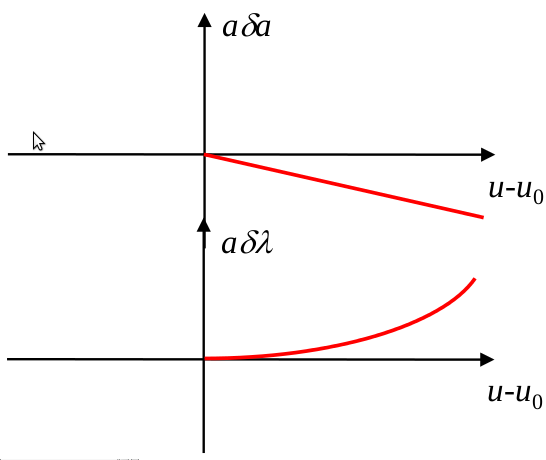
\includegraphics[width=\textwidth]{secular_drag_effects}
      \end{minipage}
    \end{figure}
    Where $v$ is the chief spacecraft's speed, $\rho$ is the density, and $\Delta B$ is the relative ballistic coefficient ($B = cd~ A/m$). The ballistic coeficient can be match to roughly $1\%$ at launch, with another $1\%$ variation during lifetime due to differential fuel consumption. This means, for LEO orbits, differential acceleration of $<10 nm/s^2$. This effects can be neglected except in the presence of safe modes or non-cooperative spacecraft (different in deputy's and chief's attitude producing different $cd$).


  \item % h) How can we incorporate impulsive maneuvers in the relative dynamics model? How can we derive closed-form deterministic impulsive maneuvering schemes? Summarize the effects of impulsive maneuvers in R, T, and N
    Impusive maneuvers can be expressed in terms of the ROE by inversion of the solution of the HCW equations, obtaining:
    \[ \begin{array}{r c c c}
      \delta a \approx & & 2 \delta v_t/(na) & \\    
      \delta \lambda \approx & -2\delta v_r/(na) & -3(u-u_M)\delta v_t/(na) & \\
      \delta e_x \approx & \delta v_r \sin{u_M}/(na) & +2\delta v_t\cos{u_M}/(na) & \\
      \delta e_y \approx & -\delta v_r \cos{u_M}/(na) & +2\delta v_t \sin{u_M}/{na} & \\
      \delta i_x \approx & & & +\delta v_n \cos{u_M}/(na) \\
      \delta i_y \approx & & & +\delta v_n \sin{u_M}/(na) 
  \end{array}\]
  where $(\delta v_r,\delta v_t,\delta v_n)$ is the relative velocity obtain with the impulsive maneuvers expresed in the chief's RTN frame. We can see that the out-of-plane maneuver is decoupled from the along-track and radial maneuvers. A close form solution can be obtain by dividing the in-plane maneuver in two seperate maneuvers.


  \item % i) Why do we aim at closed-form solution of the relative motion control problem?
    Close form solutions allow us to plan maneuvers for formation keeping over the mission lifetime or to acquire new formation geometries.

  \item % j) Describe the closed-form minimum delta-v solution for out-of-plane control, both geometrically and analytically
    For out-of-plane maneuver, the $\delta v_n$ required and the maneuvre location $u_M$ in order to mantain a require $\vec{\delta i}^{man}$ are:
    \begin{figure}[h]
      \begin{minipage}{0.5\textwidth}
	\[\delta v_n = n a \norm{\vec{\delta i}^{man}-\vec{\delta i}} \]
	\[ u_M = \tan{\frac{\vec{\delta i_y}^{man}-\vec{\delta i_y}}{\vec{\delta i_x}^{man}-\vec{\delta i_x}}}^{-1} \]
	where $\vec{\delta i}$ is the current inclination vector. In the case of correcting J2 effects, only $\delta i_y$ varies, so the maneuver position is $u_M = \pi$.
      \end{minipage}
      \begin{minipage}{0.5\textwidth}
	\centering
	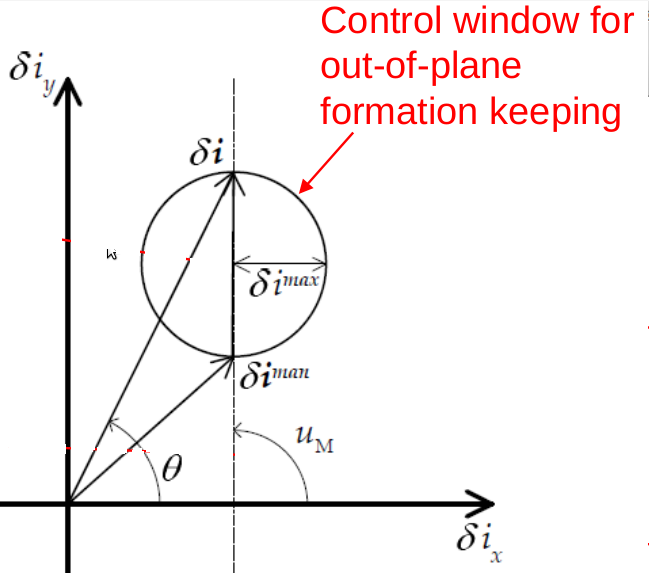
\includegraphics[width=\textwidth]{Out-of-plane_maneuvre}
      \end{minipage}
    \end{figure}

  \item % k) Describe the closed-form minimum delta-v solution for in-plane control (two pulses), both geometrically and analytically
    For in plane formation keeping, the minimum $\delta v$ two impulse solution consists in two along-track impulses separated $180^o$ in mean argument of latitud (radial impulses are less eficient). The maneuver corrects both $\delta a$ (in order to mantain a bouded orbit) and $\vec{\delta e}$:\\
    \begin{figure}[h]
    \begin{minipage}{0.5\textwidth}
      \[\delta {v_t}_1 = \frac{n a}{4} \left[ (\delta a^{man} - \delta a) + \norm{\delta e^{man} - \delta e} \right] \]
      \[\delta {v_t}_2 = \frac{n a}{4} [(\delta a^{man} - \delta a) - \norm{\delta e^{man} - \delta e}] \]
      \[{u_M}_1 = \tan{\frac{(\delta e_y^{man}-\delta e_y)}{(\delta e_x^{man} - \delta e_x)}}^{-1} \]
      \[{u_M}_2 = {u_M}_1 + \pi \]
    \end{minipage}
    \begin{minipage}{0.5\textwidth}
	\centering
	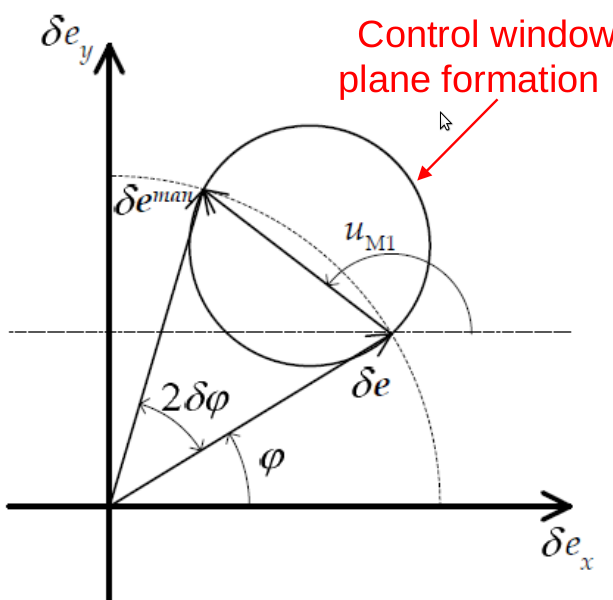
\includegraphics[width=\textwidth]{In-plane_maneuvre}
    \end{minipage}
  \end{figure}

  \item % l) Describe the closed-form minimum delta-v solution for in-plane control (three pulses), both geometrically and analytically

  \item % m) Describe how we try to generalize the closed-form solution approach for large reconfigurations including perturbations

\end{enumerate}



\section{Questions 4.2}

\section{Questions 5.1}

\section{Questions 5.2}
\begin{enumerate}[label=\emph{\alph*)}]
  \item % a) List some key metrology systems used for spacecraft formation-flying and rendezvous.
    The key metrology systems used for spacecraft formation-flying and rendezvous are:
    \begin{itemize}
      \item Gyrometer Assembly: provides angular rates for attitude determination.
      \item Accelerometer Assembly: monitors ATV boosts.
      \item Two Star Sensors for absolute attitude information.
      \item Two telegoniometers: lasers with two mirrors for beam steering.
      \item Two vidiometers.
      \item GPS/GNSS.
      \item Radio frequency:provides GPS like signals for relative navigation, applicable for deep space navigation.
      \item Vision-based systems.
    \end{itemize}

  \item % b) Why do we need relative navigation? Is it always to serve the needs of an automatic control system?
    We could need relative navigations for any mision involving two spacecraft, independently of the existance of a automatic control system. We could use relative navigation to improbe orbit determination and better plan future manouvers (no need to be automatize).

  \item % c) What are the two basic processing methods for absolute/relative orbit determination? Which are more suited to on-board and on-ground implementation? Advantages and disadvantage? Why don’t we usually use deterministic methods?
    The two basic methods for relative/absolute orbit determination are:
    \begin{itemize}
      \item Sequential estimation, where a new estimate of the state vector is obtained after each obsevation, suited for on board implementation. This method converge more quickly at the cost of stability. Also, it is more sensitive to bad lectures.
      \item Batch estimation, where all observations are processed and combined to obtain a single update state vector. This method is best suited for an on-ground implementations, where the state vector can be less frequently updated.
    \end{itemize}
  
  \item % d) What is the most common filter used for on-board navigation? What are the assumptions behind this filter? What is the difference between the time and measurement udpates? What are the key ingredients necessary to implement the filter?
    Deterministic methods are not use because they are no able to account for uncertainties and include more state parameters.(But why?)

  \item The most common filter used for on-board navigation is the Kalman Filter, which relays on the assumption that meassurements are unbiased and timewise uncorrelated (meassurement error in time $T+1$ is not affected by meassurement in time $T$. Time updates of both the state vector and covariance matices is done using a propagation matrix $\Phi$ based in the linearization of the dinamic equations. $\Phi$ is calculated based on the state values of the previos time. Measurement update are done comparing new measurements with estimated measurements based on previos measurements propagated through time. The merge between propagated measurements and new measurements is done using the gain matrix $K$, calculated from the correlation matrix propagated, the uncertainty matrix of the meassurements, and the partial derivative of the measurement to state vector matrix $H$. The key ingrediants of this filter are:
    \begin{itemize}
      \item Dynamical model.
      \item Measurement model.
      \item Uncertainty state estimate.
      \item Uncertainty of measurements.
      \item Uncertainty of dynamics.
      \item Loss function to be minimized.
    \end{itemize}

  \item The main change in the filter due to a change in the measurements type would be in the measurement model $h$ and the partial derivatives of the measurements with respect to the state vector, $H$. For example:
    
  \item The goal of TAFF system is to determine the micro-thruster commands in order to keep correct fly formation in the orbit intrack-radial plane (orbit plane) using navegation data from GNSS, and to provide the rest of the system predicted minimim separation and relative position and velocity. TAFF also handles ground planned maneuvers for absolute orbit control, which are used to better propagate meassurements, and to assure no overlaping between both controls.
  \item The state representation for the relative motion used are the relative osculating orbit parameters (in fact, due to the close position of both spacecraft, we can assume without much error that mean and osc. relative orbit elements are similar).
    $write state representation vector$\\
    The observer measures relative position and velocity (measured and express in the ECEF frame). The perturbations taken into account are $J_2$ secular perturbations, throuth the $3\gamma\sin{i}^2$, $-12\gamma \sin{2i}$ and $\dot{\phi}$ terms in the transition matrix $\Phi=\frac{\partial \Delta \alpha (t)}{\partial \Delta \alpha (t_0)}$.

  \item In order to compute the relative position and velocity in the RTN frame directly from the ECEF data is:
\end{enumerate}

\section{Questions 6.1}

\section{Questions 6.2}



\end{document}

